\section{}
Zbudowano funkcję logiczną dla segmentu C wskaźnika 7-segmentowego z wykorzystaniem bramek NAND, przy założeniu wyświetlania  liczb w systemie ósemkowym.
Segment C jest nie aktywny tylko w przypadku wyświetlania liczby \(2_8 = 010_2\).
Oznaczając kolejne bity (od najstarszego) A, B i C, a następnie przekształcając do postaci iloczynowej z użyciem praw de Morgana otrzymujemy:

\begin{align}
    Y & = A + \overline{B} + C                                      \\
    Y & = \overline{\overline{A} \cdot \overline{C}} + \overline{B} \\
    Y & = \overline{\overline{A} \cdot B \cdot \overline{C}}
\end{align}

\begin{figure}[H]
    \centering
    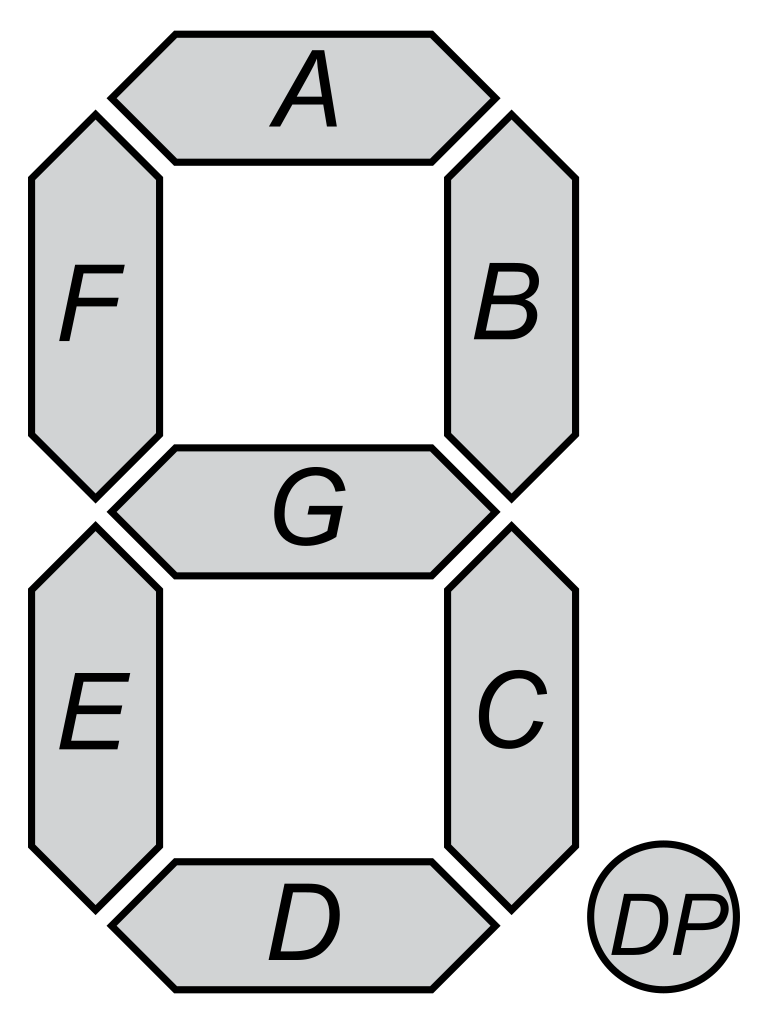
\includegraphics[width=2cm]{include/5/7seg.png}
    \caption{Oznaczenie segmentów wskaźnika 7-segmentowego. Kropka (DP) nie jest rozpatrywana.}
\end{figure}

\begin{figure}[H]
    \centering
    \begin{circuitikz}
        \draw
        (0, 1) node(gate1)[nand port] {}
        (2, 0) node(gate2)[nand port] {};

        \draw
        (gate1.in 1) to[short,-*] ++(-1, 0)
        node[anchor=east] {A}
        (gate1.in 2) to[short,-*] ++(-1, 0)
        node[anchor=east] {C}
        (gate2.in 2) to[short,-*] ++(-3, 0)
        node[anchor=east] {B};

        \draw
        (gate1.out) to[short,-] (gate2.in 1 |- gate1.out)
        to[short,-] (gate2.in 1);

        \draw
        (gate2.out) to[short,-*] ++(1, 0)
        node[anchor=west] {Y};
    \end{circuitikz}
    \caption{Schemat układu zbudowanego z bramek NAND realizującego zadaną funkcję logiczną.}
\end{figure}
